\documentclass[a4paper,12pt]{article}
%\usepackage{latexsym}
%\usepackage[MeX]{polski}
%\usepackage[latin2]{inputenc}% ew. utf8 lub cp1250
\usepackage{enumitem}
%\usepackage{nopageno}
\usepackage{geometry}
\usepackage{graphicx}
\usepackage{wrapfig}
\usepackage{xcolor}
\usepackage[square,sort&compress,comma,numbers]{natbib}
\usepackage{iopams}
\usepackage{amsmath}
\usepackage[ruled,vlined]{algorithm2e}
\newgeometry{tmargin=1.5cm, bmargin=1.5cm, lmargin=2.5cm, rmargin=2.5cm}
\newcommand{\rmd}{\mathrm{d}}
\bibliographystyle{sms}
% Zdefiniowanie autora i~tytułu:
\author{Piotr Fiborek}
%\date{}
\title{Numerical analysis of Guided Waves propagation in Honeycomb Sandwich Composites\\
(\textit{Analiza numeryczna propagacji fal prowadzonych w wielowarstwowych materia\l{}ach przek\l{}adkowych z rdzeniem o strukturze plastra miodu})}
\begin{document}
\maketitle
\thispagestyle{empty}
\section{Introduction}
\label{sec:intro}
Honeycomb Sandwich Composite~(HSC) is a type of multi-layered structure, which 
is composed of the mid-core with the geometry of honeycomb sandwiched between 
thin skins.
They are widely used in the aerospace, marine and automotive industries due to 
the high strength-to-weight ratio, high energy absorption capability and 
effective acoustic insulation.
However, these complex structures are exposed to various types of damage that are not found in metal alloy materials, e.g. hidden disbonds between the skin and the core, delamination of the skin plates, or the core impact damage.
They can occur either during a manufacturing process, storage or in-service life.
Because of this, advanced methods are required for on-line damage detections.

The structural health monitoring (SHM) method with very high potential is the method based on the Guided Wave (GW) propagation \cite{mustapha2011assessment, sikdar2016guided, sikdar2016ultrasonic,radzienski2016assessment, yu2019core}.
GW are mechanical waves that propagate in a bounded, elastic medium, e.g. bars, 
beams, rods, plates and shells.
Excitation and sensing of the GW can be realised by the lightweight and inexpensive piezoelectric transducers (PZT) \cite{giurgiutiumicromechatronics}.
The compact PZT can be surface-bonded to the inspected structure or even embedded between the composite plies so that the measurements can be conducted in situ. Among numerous techniques developed for damage detection and localisation, the most popular are pitch{catch \cite{ihn2008pitch, sikdar2017structural}, pulse--echo \cite{guo1993interaction, kudela2008damage}, phase array \cite{lu2006crack, ostachowicz2008elastic}, and time-reversal mirror \cite{fink1992time, eremin2016analytically}.

The most common numerical modelling of the phenomenon of GW in HSC found in the literature is a calculation of the effective material properties of the 
honeycomb structure by the homogenisation process~\cite{shi1995derivation, qi2008ultrasonic, mustapha2014leaky, baid2015dispersion, sikdar2016guided}.
However, this method is not able to adequately present the phenomenon of 
propagation of elastic waves in such material.
A more accurate model will be achieved if the real geometry of the hexagonal 
cell is retained.

Ruzzenne et al. presented a parametric study to evaluate the dynamic behavior of the honeycomb and cellular structures through the finite element model 
and the application of the theory of periodic structures \cite{ruzzene2003wave}.
Recently, the simulations of the wave propagation in the HSC have been conducted 
with the commercially available finite element code~\cite{song2009guided, 
hosseini2013numerical, tian2015wavenumber, zhao2018wave}.
However, finite element simulations (FEM) of GW are inefficient as they require 
significant amounts of memory and are time-consuming.

The computational efficiency of the FEM in case of GW modelling in the HSC can be improved by using the time-domain spectral element method (SEM).
The SEM was originally used for the numerical solution of the fluid flow 
in a channel by Patera \cite{patera1984spectral} but has also been successfully developed for elastic wave propagation~\cite{ostachowicz2011guided}. 
Kudela proposed a model of the GW in HSC by the parallel implementation of the SEM \cite{kudela2016parallel}.
However, this model had a large number of degree-of-freedom (DOF), because cells of the core and skin plate were modelled by the three-dimensional (3D) spectral elements.
Therefore, the simulation was limited to only one skin plate and the small dimension of the HSC (\(179 \times 159 \) mm).

Above mentioned drawbacks were motivation to propose a new model of the HSC. 
In the present paper, the skin plates, adhesive layers and each wall of the hexagonal core were modelled by two-dimensional (2D) spectral elements.
The displacements of each cell are calculated in the local coordinate system, 
and then, through the transformation matrix, they are transformed into the 
global coordinate system.
Subsequently, the core is connected to the skin plates so that displacements of 
common geometrical points of both elements are the same in each direction of 
the main axes.
This type of connection is implemented by means of interface elements based on 
Lagrange multipliers, which are interpreted as forces responsible for 
determining the appropriate displacements of nodes.
By using the interface, it is possible to model skin plates with 2D elements.
This type of approach will reduce the number of degrees of freedom, which in 
turn will shorten the calculation time and reduce the need for operational 
memory.

Signal excitation and receiving were realised by the piezoelectric (PZT) transducers, which was modelled by a three-dimensional (3D) spectral element with the electromechanical coupling.
\section{The time-domain spectral element method formulation}
\label{sec:time_SEM}
\subsection{The spectral element method}
\label{sec:sem}
The general concept of the SEM is based on the idea of the FEM.
The similarity of both methods lies in the fact that the modelled domain is divided into non-overlapping finite elements, and external forces and arbitrary boundary conditions are imposed in the particular nodes.
The main difference between those methods is a choice of the shape function \( N=N(\xi )\), which is interpolated by Lagrange polynomial that passes through the element nodes. The nodes are localized on the endpoint of an interval, \(\xi\in[-1,1]\) and the roots of the first derivative of Legendre polynomial of degree \(p-1\) (see Eq.~(\ref{eq:nodes})).

\begin{eqnarray}
	(1-\xi^2)P'_{p-1}(\xi)=0
	\label{eq:nodes}
\end{eqnarray}

The approximation of integral over the elements is achieved according to Gauss-Lobatto-Legendre (GLL) rule at points coinciding with the element nodes, 
and the weights \(w=w(\xi)\) equal to Eq. \ref{eq:weights}. This approach guarantees a diagonal mass matrix.
\begin{eqnarray}
{w(\xi)} = \frac{2}{p(p-1)(P_{p-1}(\xi))^2}
\label{eq:weights}
\end{eqnarray}

The shape function and the weights for 2D or 3D elements are obtained by the Kronecker product of vectors of individual axes, denoted by \(\otimes\) as follow:
\begin{eqnarray}
N(\xi,\eta) = N(\xi)\otimes N(\eta), & N(\xi,\eta,\zeta) = N(\xi)\otimes N(\eta)\otimes N(\zeta) \nonumber\\
w(\xi,\eta) = w(\xi)\otimes w(\eta), & w(\xi,\eta,\zeta) = w(\xi)\otimes w(\eta)\otimes w(\zeta) 
\label{eq:3Dshape_weights}
\end{eqnarray}
\subsection{2D spectral modeling}
\label{sec:2D_SEM}

According to the first-order shear deformation theory~\cite{reissner1945effect, mindlin1951influence} the displacements vector is expressed as:
\begin{eqnarray}
\left [ \begin{array}{c}
\textbf{u}^e(\xi,\eta,\zeta) \\
\textbf{v}^e(\xi,\eta,\zeta) \\
\textbf{w}^e(\xi,\eta,\zeta)
\end{array} \right] = 
\left [ \begin{array}{c}
\textbf{u}_0^e(\xi,\eta) + z\boldsymbol{\varphi}_x^e(\xi,\eta)\\
\textbf{v}_0^e(\xi,\eta) + z\boldsymbol{\varphi}_y^e(\xi,\eta)\\
\textbf{w}_0^e(\xi,\eta) \\
\end{array} \right]
\end{eqnarray}
where \(\textbf{u}_0^e\), \(\textbf{v}_0^e\) and \(\textbf{w}_0^e\) denote the 
displacements of a point on the mid-plane, \(\boldsymbol{\varphi}_x^e\), 
\(\boldsymbol{\varphi}_y^e\) are the rotations of the normal to the mid-plane 
with respect to axes \textit{x} and \textit{y}, respectively.
\begin{eqnarray}
\left [ \begin{array}{c}
\textbf{u}_0^e(\xi,\eta) \\
\textbf{v}_0^e(\xi,\eta) \\
\textbf{w}_0^e(\xi,\eta) \\
\boldsymbol{\varphi}_x^e(\xi,\eta) \\
\boldsymbol{\varphi}_y^e(\xi,\eta)
\end{array} \right]
& = & \textbf{N}^e(\xi,\eta)\widehat{\textbf{d}}^e\nonumber\\
& = & \sum_{n=1}^q\sum_{m=1}^p\textbf{N}_m^e(\xi)\textbf{N}_n^e(\eta)
\left [ \begin{array}{c}
\widehat{\textbf{u}}_0^e \\
\widehat{\textbf{v}}_0^e \\
\widehat{\textbf{w}}_0^e \\
\widehat{\boldsymbol{\varphi}}_x^e \\
\widehat{\boldsymbol{\varphi}}_y^e
\end{array} \right]
\end{eqnarray}
The bending strain components can be written as~\cite{ferreira2008matlab}:
\begin{eqnarray}
\bepsilon_b^e(\xi,\eta)=\textbf{B}_b^e\widehat{\textbf{d}}^e
\end{eqnarray}
where \(\textbf{B}_b^e\) is curvature-displacement matrix calculated as:
\begin{eqnarray}
\textbf{B}_b^e=\textbf{L}_b\textbf{N}^e(\xi,\eta)
\end{eqnarray}
\begin{eqnarray}
	\textbf{L}_b=\left [
	\begin{array}{ccccc}
		\frac{\partial }{\partial x} & 0 & 0 & 0 & 0\\
		0 & \frac{\partial }{\partial y} & 0 & 0 & 0\\
		\frac{\partial }{\partial y} & \frac{\partial }{\partial x} & 0 & 0 & 0\\
		0 & 0 & 0 & -\frac{\partial }{\partial x} & 0\\
		0 & 0 & 0 & 0 & -\frac{\partial }{\partial y}\\
		0 & 0 & 0 & -\frac{\partial }{\partial y} & -\frac{\partial }{\partial x}
	\end{array} \right],\ \\
  \left [
	\begin{array}{c}
		\frac{\partial }{\partial x}\\
		\frac{\partial }{\partial y}
	\end{array} \right] =\textbf{J}^{-1}
	\left [
	\begin{array}{c}
		\frac{\partial }{\partial \xi}\\
		\frac{\partial }{\partial \eta}
	\end{array} \right], \ 
	\textbf{J}=\left [
	\begin{array}{cc}
		\partial_\xi x & {\partial_\xi y} \\
		\partial_\eta x & {\partial_\eta y}
	\end{array} \right] \nonumber
\end{eqnarray}
The shear strain components can be written as~\cite{ferreira2008matlab}:
\begin{eqnarray}
\bepsilon_s^e(\xi,\eta)=\textbf{B}_s^e\widehat{\textbf{d}}^e
\end{eqnarray}
where \(\textbf{B}_s^e\) is curvature-displacement matrix calculated as:
\begin{eqnarray}
\textbf{B}_s^e=\textbf{L}_s\textbf{N}^e(\xi,\eta)
\end{eqnarray}
\begin{eqnarray}
\textbf{L}_s=\left [
\begin{array}{ccccc}
0 & 0 & \frac{\partial }{\partial x} & -1 & 0 \\
0 & 0 & \frac{\partial }{\partial y} & 0 & -1
\end{array} \right]
\end{eqnarray}
\subsection{3D model of the PZT transducer}
\label{sec:3D_SEM}
The displacements of the PZT transducer are defined by three displacement components \textbf{u}, \textbf{v} and \textbf{w}, and can be express in a form:
\begin{eqnarray}
\left [ \begin{array}{c}
\textbf{u}^e(\xi,\eta,\zeta) \\
\textbf{v}^e(\xi,\eta,\zeta) \\
\textbf{w}^e(\xi,\eta,\zeta)
\end{array} \right]
& = & \textbf{N}^e(\xi,\eta, \zeta)\widehat{\textbf{d}}^e\nonumber\\
& = & \sum_{l=1}^r\sum_{n=1}^q\sum_{m=1}^p\textbf{N}_m^e(\xi)\textbf{N}_n^e(\eta)\textbf{N}_l^e(\zeta)
\left [ \begin{array}{c}
\widehat{\textbf{u}}^e(\xi_m,\eta_n,\zeta_l) \\
\widehat{\textbf{v}}^e(\xi_m,\eta_n,\zeta_l) \\
\widehat{\textbf{w}}^e(\xi_m,\eta_n,\zeta_l)
\end{array} \right]
\label{eq:3D_displ}
\end{eqnarray}
where \(\widehat{\textbf{u}}^e\), \(\widehat{\textbf{v}}^e\) and 
\(\widehat{\textbf{w}}^e\) are nodal values.
Six components of the strain matrix are approximated as follow 
\cite{kudela20093d}:
\begin{eqnarray}
\bepsilon^e(\xi,\eta,\zeta)=\textbf{B}_{d}^e\widehat{\textbf{d}}^e
\end{eqnarray}
where \(\textbf{B}_{d}^e\) is strain-nodal displacement matrix calculated as:
\begin{eqnarray}
\textbf{B}_{d}^e=\textbf{L}\textbf{N}^e(\xi,\eta,\zeta)
\end{eqnarray}
\begin{eqnarray}
\textbf{L}=\left [
\begin{array}{ccc}
\frac{\partial }{\partial x} & 0 & 0\\
0 & \frac{\partial }{\partial y} & 0\\
0 & 0 & \frac{\partial }{\partial z}\\
0 & \frac{\partial }{\partial z} & \frac{\partial }{\partial y}\\
\frac{\partial }{\partial z} & 0 & \frac{\partial }{\partial x}\\
\frac{\partial }{\partial y} & \frac{\partial }{\partial x} & 0
\end{array} \right],\ 
\left [
\begin{array}{c}
\frac{\partial }{\partial x}\\
\frac{\partial }{\partial y}\\
\frac{\partial }{\partial z}
\end{array} \right] =\textbf{J}^{-1}
\left [
\begin{array}{c}
\frac{\partial }{\partial \xi}\\
\frac{\partial }{\partial \eta}\\
\frac{\partial }{\partial \zeta}
\end{array} \right], \ 
\textbf{J}=\left [
\begin{array}{ccc}
\partial_\xi x & {\partial_\xi y} & {\partial_\xi z}\\
\partial_\eta x & {\partial_\eta y} & {\partial_\eta z}\\
\partial_\zeta x & {\partial_\zeta y} & {\partial_\zeta z}
\end{array} \right]
\end{eqnarray}

The electromechanical coupling is governed by the linear constitutive equation 
of piezoelectric material according to~\cite{giurgiutiumicromechatronics} and 
it is expressed by:
\begin{eqnarray}
\left [ 
\begin {array}{c}
\bsigma\\
\textbf{D}
 \end{array}\right ]=
\left [ 
\begin{array}{cc}
\textbf{c}^E & -\textbf{e}^T \\
\textbf{e} & \bepsilon^S 
\end{array} \right ]
\left[ 
\begin{array}{c}
\textbf{S}\\
\textbf{E} 
\end{array} \right ]
\end{eqnarray}
where \(\textbf{c}^E\), \textbf{e} and \(\bepsilon^S\) are tensors of elastic, 
piezoelectric and dielectric constants, respectively, \textbf{E} and \textbf{D} 
are the electric field and electric displacement, \(\bsigma\) and \textbf{S} 
are stress and strain.
The superscripts E and S indicate that quantities are measured at zero electric 
fields and zero strain, respectively and the subscript T denotes transpose 
matrix.
Electric field vector can be expressed as:
\begin{eqnarray}
\textbf{E}^e=-\textbf{B}_\phi^e \widehat{\bphi}^e
\end{eqnarray}
where \(\textbf{B}_\phi^e\) is electric-nodal potential matrix calculated as:
\begin{eqnarray}
\textbf{B}_\phi^e=
\left[ \begin{array}{c}
\frac{\partial }{\partial \xi}\\
\frac{\partial }{\partial \eta}\\
\frac{\partial }{\partial \zeta}
\end{array} \right]\textbf{N}^e(\xi,\eta,\zeta)
\end{eqnarray}

\subsection{Displacements coupling at the substructures interface}
\label{sec:interface}
The present model of the sandwich panel consists of 2D and 3D elements. 
Moreover, there are non-matching grids between two adjacent substructures. 
These involve connecting them by imposing the compatibility of the 
displacements at the interface, see Fig.~\ref{fig:interface}.
The coupling can be expressed as:
\begin{eqnarray}
\left\{\begin{array}{c}
	\textbf{u}\\
	\textbf{v}\\
	\textbf{w}
	\end{array}\right\}_{s_{i1}}^{\Gamma^i}-
	\left\{\begin{array}{c}
	\textbf{u}\\
	\textbf{v}\\
	\textbf{w}
	\end{array}\right\}_{s_{i2}}^{\Gamma^i}=
	\left\{\begin{array}{c}
	\textbf{0}\\
	\textbf{0}\\
	\textbf{0}
	\end{array}\right\}
\label{eq:coupling}
\end{eqnarray}
\begin{figure}
	\begin{center}
		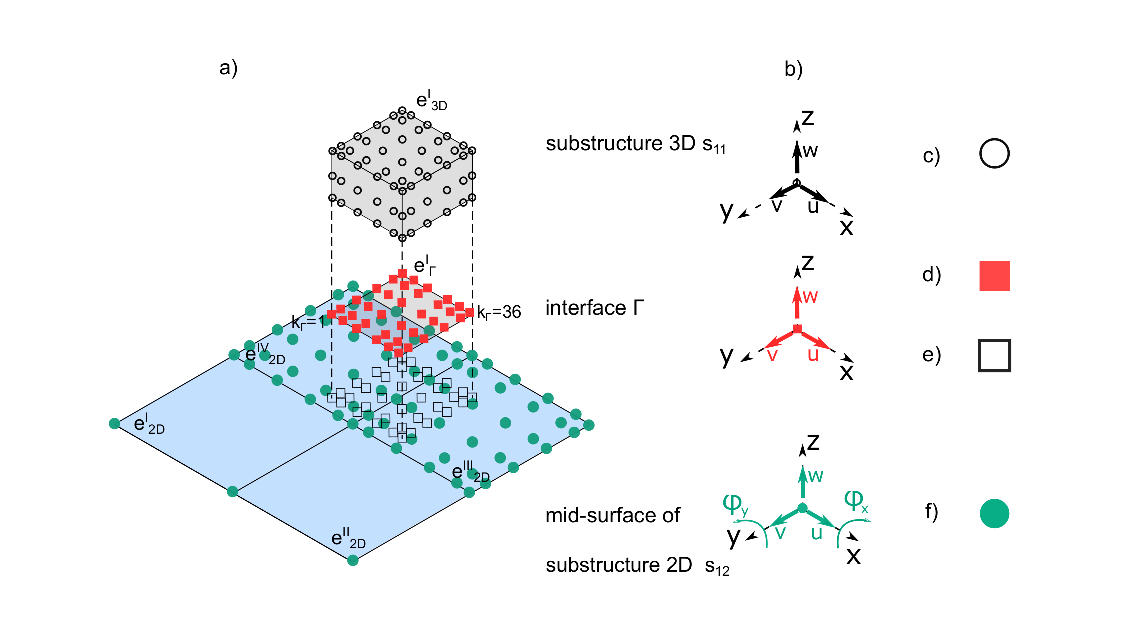
\includegraphics[width=1\linewidth]{../../../figures/eps/interface_2D3D.eps}
	\end{center}
	\caption{Interface setup: a) interface coupling, b) degrees of freedom of the interface and the substructures, c) the nodes at the bottom layer of the 3D substructure, d) the remaining nodes of the 3D substructure, e) the nodes of the interface projected to the bottom layer of the 3D 
	substructure, f) the nodes of the interface, g) the nodes of the interface projected to mid-surface of the 2D substructure, h) the nodes of the 2D substructure}
	\label{fig:interface}
\end{figure}
For the whole structure, equation~\ref{eq:coupling} can be written in the 
matrix form:
\begin{eqnarray}
\textbf{G}\textbf{d}=\textbf{0}
\label{eq:cond_disp}
\end{eqnarray}
where \textbf{G} is the coupling matrix which contains the equations to 
interpolate the substructures displacements at the interfaces, and 
\(\textbf{d}\) is a global vector of displacements for \(nS\) number of 
substructures, composed as:
\begin{eqnarray}
\textbf{d} = \left\{\begin{array}{cccc}
\textbf{d}_1, & \textbf{d}_2, &\ldots, & \textbf{d}_{nS}
\end{array}\right\}^T
\label{eq:displacements}
\end{eqnarray}

General formulation of the matrix \textbf{G} is proposed in Algorithm 
\ref{alg:G_matrix}.
The main task of the algorithm is to calculate shape functions for each 
adjacent substructures at the points \(X_p=(x_p^k,y_p^k)\), which are 
projections of the interface nodes onto these substructures.
The shape function can be calculated after finding an owner element and local 
coordinates of the points.
Owner element is a spectral element in the domain of the substructure \(s_{ij}\) which contains interface node, for example, interface node \(k=6\) 
(see~Fig.~\ref{fig:interface}a)) is located in element \(e^I\) and 
\(e^{III}\) for the substructures \(s_{i1}\) and \(s_{i2}\), respectively.
It can be found within two ways: using Matlab's built-in function 
\verb+inpolygon+ or more efficient procedure proposed by Silva et al. 
\cite{silva2009exact} which was used in the current implementation.
The transformation from global to local coordinates was realized by the 
iterative method presented in the work of Li et al.~\cite{li2014efficient}.


\begin{algorithm}[H]
	\SetAlgoLined
	\KwResult{coupling matrix \textbf{G}}
	create empty \(nI \times nS\) cell array: \(\mathbf{G} = cell(nI,nS)\)\;
	\For{i = 1 \KwTo nI}{
		find two common structures of interface \(\Gamma^i\): \(s_i = 
		(s_{i1},s_{i2})\)\;
		\For{j = 1 \KwTo 2}{
			create \(n^{\Gamma^i}\times n^{s_{ij}}\) null matrix 
			\(\mathbf{G}^{s_{ij}}_i\),\\
			\For{k = 1 \KwTo \(n^{\Gamma^i}\)} {
				find \(ownerElement^{s_{ij}}_k\) in the structure \(s_{ij}\) 
				containg interface node \(k\) with global coordinates vector: 
				\(X_p=(x^k_p,y^k_p)\)\;
				assign vector \(X_e=(x_e,y_e)\) of coordinates of all nodes in 
				\(ownerElement^{s_{ij}}_k\)\;
				assign initial coordinates 
				\(X_{\kappa}=(x^k_{\kappa},y^k_{\kappa})\) to the nearest node 
				in 
				\(ownerElement^{s_{ij}}_k\) to node \(k\)\;
				transform global coordinates \(X_{\kappa}\) to local coordinate 
				system \(\xi_{\kappa}=\xi(X_{\kappa});\quad 
				\eta_{\kappa}=\eta(X_{\kappa})\)\;
				\While{\(\left|X_p-X_{\kappa}\right|>tol\)}{
					\(\xi_{\kappa+1}=\xi_{\kappa}+(J^{-1}_{\kappa})_{11}.*(x^k_p-x_{\kappa}^k)+(J^{-1}_{\kappa})_{12}.*(y^k_p-y_{\kappa}^k)\)\;
					\(\eta_{\kappa+1}=\eta_{\kappa}+(J^{-1}_{\kappa})_{21}.*(x^k_p-x_{\kappa}^k)+(J^{-1}_{\kappa})_{22}.*(y^k_p-y_{\kappa}^k)\)\;
					\(X_{\kappa}=N(\xi_{\kappa+1},\eta_{\kappa+1})X_e\)\;
				}
				\(\xi^k_p\approx \xi_{\kappa+1},\quad \eta^k_p\approx 
				\eta_{\kappa+1}\)\;
				\(\mathbf{G}^{s_{ij}}_i(k,nX_e)=N(\xi^k_p,\eta^k_p)\)\;
			}
			\uIf{elements of \(s_{ij}\) are 3D} {
				
				\(\mathbf{G}\{i,s_{ij}\}=\left[\begin{array}{ccc}
				\mathbf{G}^{s_{ij}}_i & \mathbf{0} & \mathbf{0}\\
				\mathbf{0} & \mathbf{G}^{s_{ij}}_i & \mathbf{0}\\
				\mathbf{0} & \mathbf{0} & \mathbf{G}^{s_{ij}}_i
				\end{array} \right]
				\)\;
			}
			\ElseIf{elements of \(s_{ij}\) are 2D} {
				
				\(\mathbf{G}\{i,s_{ij}\}=\left[\begin{array}{ccccc}
				\mathbf{G}^{s_{ij}}_i & \mathbf{0} & \mathbf{0} & 
				\frac{h_{ij}}{2}\mathbf{G}^{s_{ij}}_i & \mathbf{0}\\
				\mathbf{0} & \mathbf{G}^{s_{ij}}_i & \mathbf{0} & \mathbf{0} & 
				\frac{h_{ij}}{2}\mathbf{G}^{s_{ij}}_i\\
				\mathbf{0} & \mathbf{0} & \mathbf{G}^{s_{ij}}_i & \mathbf{0} & 
				\mathbf{0}
				\end{array} \right]
				\)\;	}
			
		}
	}
	fill empty cells of array \(\mathbf{G}\) with null matrices, and convert 
	\(\mathbf{G}\) to single matrix.
	\caption{Matrix G formulation}
	\label{alg:G_matrix}
\end{algorithm}
where \(nI\) and \(nS\) are numbers of the interfaces and the structures, 
respectively; \(n^{\Gamma^i}\) and \(n^{s_{ij}}\) are numbers of nodes of the 
interface \(i\), and the structure \(s_{ij}\), respectively; \(\eta^k_p\) and  
\(\xi^k_p\) are local coordinates of \(X_p\), respectively; \(J_{\kappa}\) is 
Jacobians evaluated at \((\xi_{\kappa+1},\eta_{\kappa+1})\) and 
\(N(\xi_{\kappa+1},\eta_{\kappa+1})\) is a shape function evaluated at 
\((\xi_{\kappa+1},\eta_{\kappa+1})\), \(nX_e\) is a vector of global order 
numbers of all nodes in the \(ownerElements^{s_{ij}}_k\), \(h_{ij}\) is a 
thickness of the structure \(s_{ij}\) and \(tol\) is a termination criterion 
for iterations.

The computational effectiveness of Algorithm~\ref{alg:G_matrix} can be 
easily improved if certain precautions are taken.
Firstly, the mesh of the interface has to be based on the mesh from one of the 
substructures \(s_i1\), \(s_i2\), which may be referred to as a slave.
So, the shape function takes only the values of one and zeros.
Moreover, the code can be implemented in vectorized form rather than using a 
for-loops.

\subsection{Elementary governing equations of motion}
\label{sec:motion}
The elementary governing equations of motion with Lagrange multipliers can be written in the matrix form:
\begin{eqnarray}
\left[
\begin{array}{ccc}
\textbf{M}_{dd} & 0 & 0\\
0 & 0 & 0\\
0 & 0 & 0
\end{array} \right]
\left \{
\begin{array}{c}
\ddot{\widehat{\textbf{d}}}\\
\ddot{\widehat{\bphi}}\\
0
\end{array} \right \}+
\left[
\begin{array}{ccc}
\textbf{C}_{dd} & 0 & 0\\
0 & 0 & 0\\
0 & 0 & 0
\end{array} \right]
\left \{
\begin{array}{c}
\dot{\widehat{\textbf{d}}}\\
\dot{\widehat{\bphi}}\\
0
\end{array} \right \}+\nonumber\\
+\left[
\begin{array}{ccc}
\textbf{K}_{dd} & \textbf{K}_{d\phi} & {\textbf{G}}^T\\
\textbf{K}_{\phi d} & \textbf{K}_{\phi \phi} & 0\\
\textbf{G} & 0 & 0
\end{array} \right]
\left \{
\begin{array}{c}
\widehat{\textbf{d}}\\
\widehat{\bphi}\\
\blambda
\end{array} \right \}=
\left \{
\begin{array}{c}
\textbf{F}\\
\textbf{Q}\\
0
\end{array} \right \}
\label{eq:motion}
\end{eqnarray}
where \(\textbf{M}_{dd}\), \(\textbf{C}_{dd}\), \(\textbf{K}_{dd}\) are 
structural mass, damping and stiffness matrices, respectively; 
\(\textbf{K}_{\phi 
d}={\textbf{K}_{d\phi}}^T\) are piezoelectric coupling matrix; 
\(\textbf{K}_{\phi 
\phi}\) is the dielectric permittivity matrix, \(\widehat{\textbf{d}}\) is the 
nodal displacements and \(\widehat{\bphi}\) is the electric potential; 
\(\textbf{F}\) the nodal external force vector, \(\textbf{Q}\) is the nodal 
externally applied charge vector, \(\blambda\) is the vector of Lagrange 
multipliers, and \(\textbf{G}\) is the Lagrange multiplier matrix; \((\dot{\ 
})=\frac{\partial}{\partial t}\).
The formulae of matrices are provided in App.~\ref{app:matrices}.
The coupling is realized by imposing the traction forces, represented by a vector of Lagrange multipliers. 

\subsection{Transformation of the core elements}
\label{sec:transformation}
All core elements are rotated relative to both skins, so it is necessary to transform degrees of freedom from the local core's coordinate system to the global system.
For this purpose, an additional sixth global dof has been incorporated, i.e. rotation with respect to the z-axis.
Firstly, a part of mass matrix accounted for rotary inertia (see App. \ref{app:matrices}) is globalised as follow:
	\begin{eqnarray}
		\textbf{M}_R^g=\textbf{a}\,\textbf{M}_R^l\,\textbf{a}^{-1}
		\label{eq:inertia}
	\end{eqnarray}
where \(\textbf{a}\) is general rotation matrix obtained from multiplication of basic rotation matrices, and for the regular hexagonal core a is equal to:
\begin{eqnarray}
	\textbf{a}=\left [ 
	\begin{array}{ccc}
	m & -n & 0\\
	0 & 0 & -1\\
	n & m & 0\\
	\end{array}
	\right ]
\label{eq:rotation}
\end{eqnarray}
where \(m=\cos(\alpha),\:n=\sin(\alpha)\), for \(\alpha\in{(0^\circ,\,60^\circ,\,120^\circ,180^\circ,\,240^\circ,\,300^\circ)}\) depending on which wall of the cell it is applied to.

The stiffness--strain relationship in local and global frame is given by:
\begin{eqnarray}
\begin{array}{ccc}
\left [
\begin{array}{c}
\sigma^l_{11}\\
\sigma^l_{22}\\ 
\sigma^l_{33}\\ 
\sigma^l_{23}\\
\sigma^l_{13}\\
\sigma^l_{12}\\
\end{array}
\right ]=
\textbf{c}\,\left [
\begin{array}{c}
\epsilon^l_{11}\\
\epsilon^l_{22}\\ 
\epsilon^l_{33}\\
\gamma^l_{23}\\
\gamma^l_{13}\\
\gamma^l_{12}\\
\end{array}
\right ], & and &
\left [
\begin{array}{c}
\sigma^g_{11}\\
\sigma^g_{22}\\ 
\sigma^g_{33}\\ 
\sigma^g_{23}\\
\sigma^g_{13}\\
\sigma^g_{12}\\
\end{array}
\right ]=
\bar{\textbf{c}}\,\left [
\begin{array}{c}
\epsilon^g_{11}\\
\epsilon^g_{22}\\ 
\epsilon^g_{33}\\
\gamma^g_{23}\\
\gamma^g_{13}\\
\gamma^g_{12}\\
\end{array}
\right ]
\end{array}
\label{eq:stress_global}
\end{eqnarray}
The global form of stiffness matrix \(K\), involves the determination of stiffness tensor \(\bar{c}\) from Eq.~\ref{eq:stress_global}.
The transformation of the stress tensor is expressed as:
\begin{eqnarray}
\left [ 
\begin{array}{ccc}
\sigma^g_{11} & \sigma^g_{12} & \sigma^g_{13}\\
\sigma^g_{21} & \sigma^g_{22} & \sigma^g_{23}\\
\sigma^g_{31} & \sigma^g_{32} & \sigma^g_{33}\\
\end{array}
\right ]
=
\textbf{a}\,
\left [ 
\begin{array}{ccc}
\sigma^l_{11} & \sigma^l_{12} & \sigma^l_{13}\\
\sigma^l_{21} & \sigma^l_{22} & \sigma^l_{23}\\
\sigma^l_{31} & \sigma^l_{32} & \sigma^l_{33}\\
\end{array}
\right ]
\,\textbf{a}^T
\label{eq:sigma_tensor}
\end{eqnarray}
After multiplication of matrices and using the symmetry of the stress tensor Eq.~\ref{eq:sigma_tensor} can be rewritten in simplified form:

\begin{eqnarray}
\left [
\begin{array}{c}
\sigma^g_{11}\\
\sigma^g_{22}\\ 
\sigma^g_{33}\\ 
\sigma^g_{23}\\
\sigma^g_{13}\\
\sigma^g_{12}\\
\end{array}
\right ]=
\textbf{T}\,\left [
\begin{array}{c}
\sigma^l_{11}\\
\sigma^l_{22}\\ 
\sigma^l_{33}\\
\sigma^l_{23}\\
\sigma^l_{13}\\
\sigma^l_{12}\\
\end{array}
\right ]
\label{eq:stress}
\end{eqnarray}

Analogously, strain relationship also is given in the form:
\begin{eqnarray}
\begin{array}{ccc}
\left [
\begin{array}{c}
\epsilon^g_{11}\\
\epsilon^g_{22}\\ 
\epsilon^g_{33}\\ 
\epsilon^g_{23}\\
\epsilon^g_{13}\\
\epsilon^g_{12}\\
\end{array}
\right ]=
\textbf{T}\,\left [
\begin{array}{c}
\epsilon^l_{11}\\
\epsilon^l_{22}\\ 
\epsilon^l_{33}\\
\epsilon^l_{23}\\
\epsilon^l_{13}\\
\epsilon^l_{12}\\
\end{array}
\right ], & and & \left [
\begin{array}{c}
\epsilon_{11}\\
\epsilon_{22}\\ 
\epsilon_{33}\\ 
\gamma_{23}\\
\gamma_{13}\\
\gamma_{12}\\
\end{array}
\right ]=
\textbf{R}\,\left [
\begin{array}{c}
\epsilon_{11}\\
\epsilon_{22}\\ 
\epsilon_{33}\\
\epsilon_{23}\\
\epsilon_{13}\\
\epsilon_{12}\\
\end{array}
\right ]
\end{array}
\label{eq:strain}
\end{eqnarray}
where \(\textbf{R}\) is the Reuter's matrix, defined as:
\begin{eqnarray}
\textbf{R} = \left [
\begin{array}{cccccc}
1 & 0 & 0 & 0 & 0 & 0\\
0 & 1 & 0 & 0 & 0 & 0\\
0 & 0  & 1 & 0 & 0 & 0\\
0 & 0 & 0 & 2 & 0 & 0\\
0 & 0 & 0 & 0 & 2 & 0\\
0 & 0 & 0 & 0 & 0 & 2
\end{array}
\right ]
\label{eq:reuters}
\end{eqnarray}
Using the Eqs.~\ref{eq:rotation} through \ref{eq:reuters} the relationship of stress--strain in the global frame can be expressed as:
\begin{eqnarray}
\left [
\begin{array}{c}
\sigma^g_{11}\\
\sigma^g_{22}\\ 
\sigma^g_{33}\\ 
\sigma^g_{23}\\
\sigma^g_{13}\\
\sigma^g_{12}\\
\end{array}
\right ]=
\textbf{T}\,\textbf{c}\,\textbf{R}\,\textbf{T}^{-1}\,\textbf{R}^{-1}\,
\left [
\begin{array}{c}
\epsilon^g_{11}\\
\epsilon^g_{22}\\ 
\epsilon^g_{33}\\
\gamma^g_{23}\\
\gamma^g_{13}\\
\gamma^g_{12}\\
\end{array}
\right ]
\label{eq:stress-strain}
\end{eqnarray}
Therefore, transformed stiffness tensor for the core's elements is equal:
\begin{eqnarray}
\bar{\textbf{c}}=\textbf{T}\,\textbf{c}\,\textbf{R}\,\textbf{T}^{-1}\,\textbf{R}^{-1}
\label{eq:c_global}
\end{eqnarray}


\subsection{Time integration of the equation of motion}
\label{sec:time_integration}
Using a central difference scheme, equation (\ref{eq:motion}) can be rewritten as follow:
\begin{eqnarray}
\left(\frac{1}{\Delta t^2}\textbf{M}_{dd}+\frac{1}{2\Delta t}\textbf{C}_{dd} \right)\widehat{\textbf{d}}_{t+\Delta t}=
\textbf{F}_t+\textbf{K}_s\bphi_t^P-\left( \textbf{K}_{dd}-\textbf{K}_a\right)\widehat{\textbf{d}}_t\nonumber\\
+\frac{2}{\Delta t^2}\textbf{M}_{dd}\widehat{\textbf{d}}_t-\left(\frac{1}{\Delta t^2}\textbf{M}_{dd}-\frac{1}{2\Delta t}\textbf{C}_{dd}\right)\widehat{\textbf{d}}_{t-\Delta t}-\textbf{G}^T\blambda_t
\label{eq:CDE}
\end{eqnarray}
where  \(\textbf{K}_s=\textbf{K}_{d\phi}^A{\textbf{K}_{\phi 
\phi}^{A,A}}^{-1}\textbf{K}_{\phi \phi}^{A,P}-\textbf{K}_{d\phi}^P\), 
\(\textbf{K}_a=\textbf{K}_{d \phi}^A{\textbf{K}_{\phi 
\phi}^{A,A}}^{-1}\textbf{K}_{\phi d}^A\), 
and \(\Delta t\) is the time increment. 
\(\textbf{K}_{d \phi}^A\) and \(\textbf{K}_{d\phi}^P\) are sub-matrices of 
matrix 
\(\textbf{K}_{d\phi}\), 
while \(\textbf{K}_{\phi \phi}^{A,P}\) and \(\textbf{K}_{\phi \phi}^{A,A}\) are 
the sub-matrices of matrix \(\textbf{K}_{\phi \phi}\).
Their formulation is realized by discarding appropriate rows and columns 
according to imposed electrical boundary conditions. \(\textbf{K}_{d \phi}^P\) 
contains columns selected from \(\textbf{K}_{d\phi}\) by vector \textbf{P}, and 
\(\textbf{K}_{d\phi}^A\) contains columns selected from \(\textbf{K}_{d\phi}\) 
by vector \textbf{A}. 
\(\textbf{K}_{\phi \phi}^{A,P}\) contains columns from \(\textbf{K}_{\phi 
\phi}\) selected by vector \textbf{P} and rows from the same matrix selected by 
vector \textbf{A}, and \(\textbf{K}_{\phi \phi}^{A,A}\) contains rows and 
columns selected from \(\textbf{K}_{\phi \phi}\) by vector \textbf{A}.
Where \textbf{P} is a list of nodes assigned to the electrodes, and \textbf{A} 
is a complement of \textbf{P} in the set of all nodes of the PZT.

Unknown Lagrange multiplier vector \(\blambda_t\) is dependent on the load 
acting on the structure, and it is calculated for each time step from 
Eq.~(\ref{eq:CDE}) by imposing the constraint Eq.~(\ref{eq:cond_disp}).
\begin{eqnarray}
\blambda_t &= &{\left(\textbf{G}\textbf{L}_+^{-1}\textbf{G}^T \right)}^{-1}\textbf{G}\textbf{L}_+^{-1} \Bigg[ \textbf{F}_t+\textbf{K}_s\bphi_t^P\nonumber\\
& & +\left.\left(\frac{2}{\Delta t^2}\textbf{M}_{dd}-\textbf{K}_{dd}+\textbf{K}_a\right)\textbf{d}_t -\textbf{L}_-\textbf{u}_{t-\Delta t} \right]
\end{eqnarray}
where \(\textbf{L}_+=\frac{1}{\Delta t^2}\textbf{M}_{dd}+\frac{1}{2\Delta 
t}\textbf{C}_{dd}\) and \(\textbf{L}_-=\frac{1}{\Delta 
t^2}\textbf{M}_{dd}-\frac{1}{2\Delta t}\textbf{C}_{dd}\).

\section{Numerical simulations}
\label{sec:numerical}
\subsection{Sample configuration}
\label{sec:sample}
The sample consists of aluminum honeycomb attached between two carbon fiber 
reinforced polymer (CFRP) plates by the adhesive layers 
(Fig.~\ref{fig:honeycomb}a)).
Material properties used in the simulations are gathered in 
App.~\ref{app:properties}.
One pair of circular PZT transducers were mounted on the top skin to generate 
and receive of guided waves signals.
Glue under the transducers were not considered.

In the middle of the structure, the circular area of the adhesive layer between 
the bottom skin and core was removed to simulate the disbonds in the HSC.
This model is simple for implementation and does not effect on the convergence of the time integration.
However, it does not take into account the contact between the structures, so the nodes of particular elements in this area may intersect with each other.
The size of the disbonds was the subject of the parametric study aiming at 
finding the damage effect on GW propagation.

The following dimensions and parameters were assumed:
\begin{itemize}
	\item CFRP skins --- L = 500, W = 314, H = 1 mm, fibers volume fraction 
	50\%, stacking sequence 
	\([0^\circ,90^\circ,0^\circ,90^\circ,0^\circ,90^\circ,0^\circ,90^\circ]\),
	\item Core --- \(\Phi\) = 19, h = 10, w = 0.07 mm 
	(Fig.~\ref{fig:honeycomb}b)),
	\item Adhesive --- L = 500, W = 314, H = 0.5 mm,
	\item PZT --- \(\Phi\) = 10, h = 0.5 mm, location \#1 \((x_1,y_1)=(-80,0)\) 
	mm,	\#2 \((x_2,y_2)=(80,0)\) mm,
	\item Disbonds \(\Phi = \left [0, 20, 40, 60, 80, 100, 120 \right ]\).
\end{itemize}

\begin{figure}
	\begin{center}
		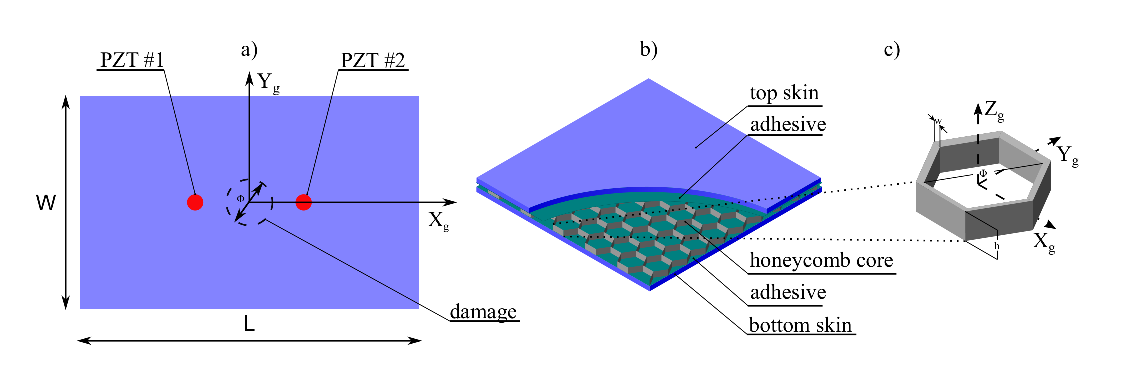
\includegraphics[width=1\linewidth]{../../../figures/eps/honeycomb.eps}
	\end{center}
	\caption{Sample configuration: a) top view of the sample, b) honeycomb sandwich substructures, c) detail of the honeycomb cell}
	\label{fig:honeycomb}
\end{figure}

\subsection{Simulation parameters}
\label{sec:simulation}
The present model is composed of \(4 \times 4\) and \(4 \times 4 \times 4\) node spectral elements for 2D and 3D components, respectively.
To decrease the number of non-zero values of the \(\textbf{G}\)~matrix, the following steps had been taken during the preparation of the mesh.
One spectral element covers the wall of the honeycomb core, while the meshes of the skin plates and the adhesive layers were divided by elements in the shape of a rhombus, three per area under each cell.
In this way, the interface nodes coincide with the nodes lying on the hexagon edges (thick line on Fig. \ref{fig:skin_mesh} b)).
In the case of PZT transducers, the mesh was generated by using external GMSH software \cite{geuzaine2009gmsh} (see Fig.~\ref{fig:skin_mesh} c)).
The prepared meshes ensure at least 6 nodes per wavelength.
\begin{figure}
	\begin{center}
		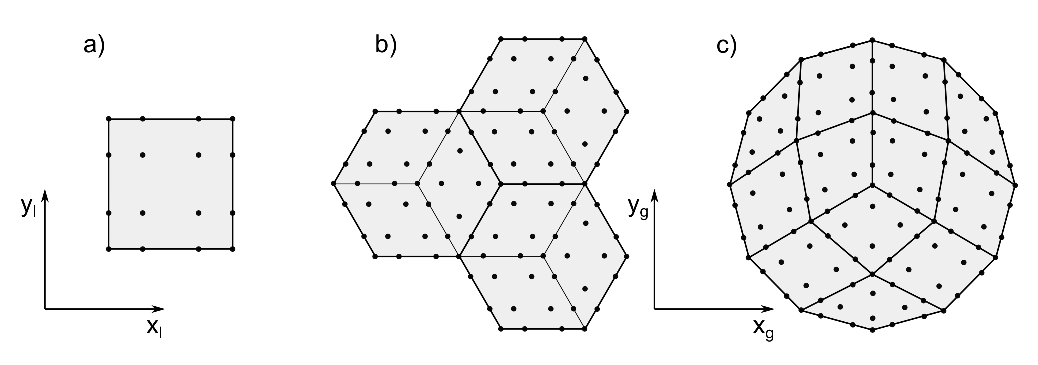
\includegraphics[width=1\linewidth]{../../../figures/eps/skin_mesh.eps}
	\end{center}
	\caption{The mesh with the nodes distribution, a) spectral element of the core's wall, b) excerpt of the skin plate, c) top view of the PZT transducer mesh}
	\label{fig:skin_mesh}
\end{figure}

The analysis was conducted with the wide bandwidth chirp signal (Fig.~\ref{fig:chirp}).
Total calculation time was set to 2 ms with time increment \(\Delta 
t=10\) ns.
The assigned excitation signal had the significant values in frequency domain between 0 and 20 kHz with resolution of 500 Hz.
\begin{figure}
	\begin{center}
		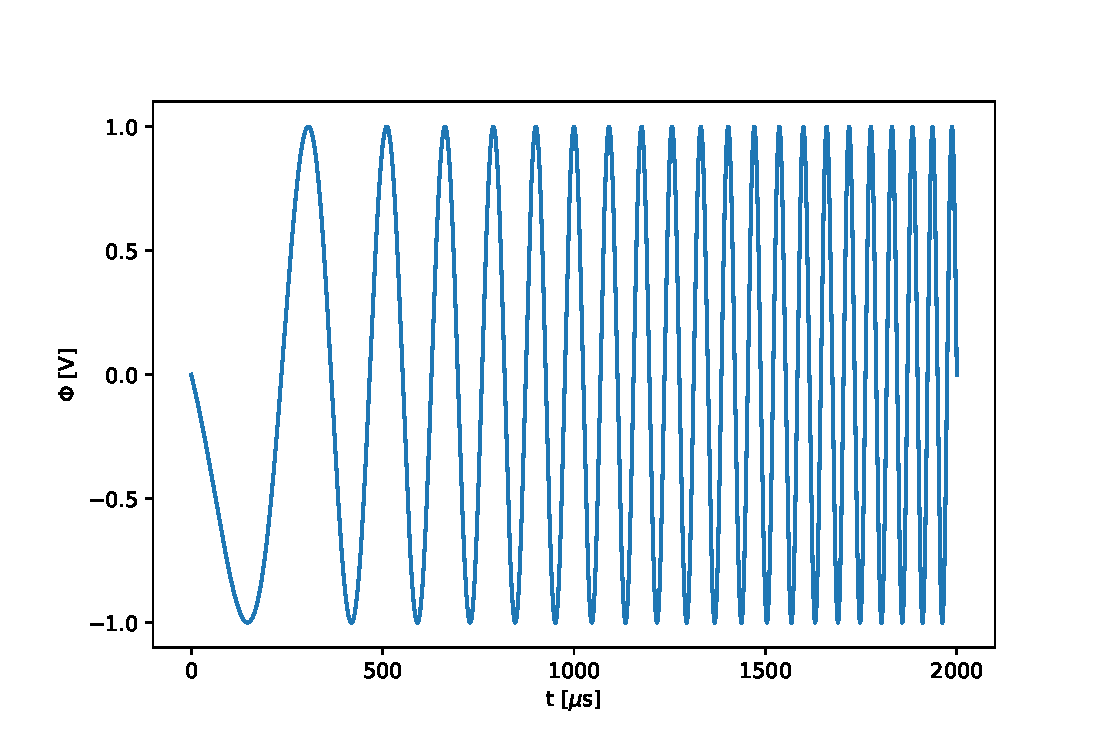
\includegraphics[width=1\linewidth]{../../../figures/eps/chirp_0_20.eps}
	\end{center}
	\caption{Chirp signal}
	\label{fig:chirp}
\end{figure}

\section{Results}
\label{sec:results}
The wave propagating through the sample interact with damage boundary, so the amplitude of the transmitted wave is expected to vary according to the size of the failure.
One can observe on the Fig. \ref{fig:wavefield} that only a portion of the wave reached the sensor, while part of the wave is entrapped within the damage. Besides, the wave also interacts with the cells, due to modelling with respect to the real geometry of the core.
\begin{figure}
	\begin{center}
		\includegraphics[width=1\linewidth]{../../../figures/eps/wavefield.eps}
	\end{center}
	\caption{Full wavefield}
	\label{fig:wavefield}
\end{figure}

To determine the effect of the damage size on GW propagation, the signal obtained by the sensor was taken into account.
The signal represents an average value of the electrical potential of the nodes belonging to the upper layer of the sensor, calculated in each time step for different damage diameter.
For further analysis, the time domain characteristics were transformed to frequency domain by the discrete Fourier transform, \(\Phi(f)=DFT(\Phi(t))\).
It can be noticed on the Fig. \ref{fig:signals}a) that the signals values do not always decrease with the increasing of damage diameter.
Therefore the MADIF is only defined for the frequency in which the function is monotonous.
\begin{figure}
	\begin{center}
		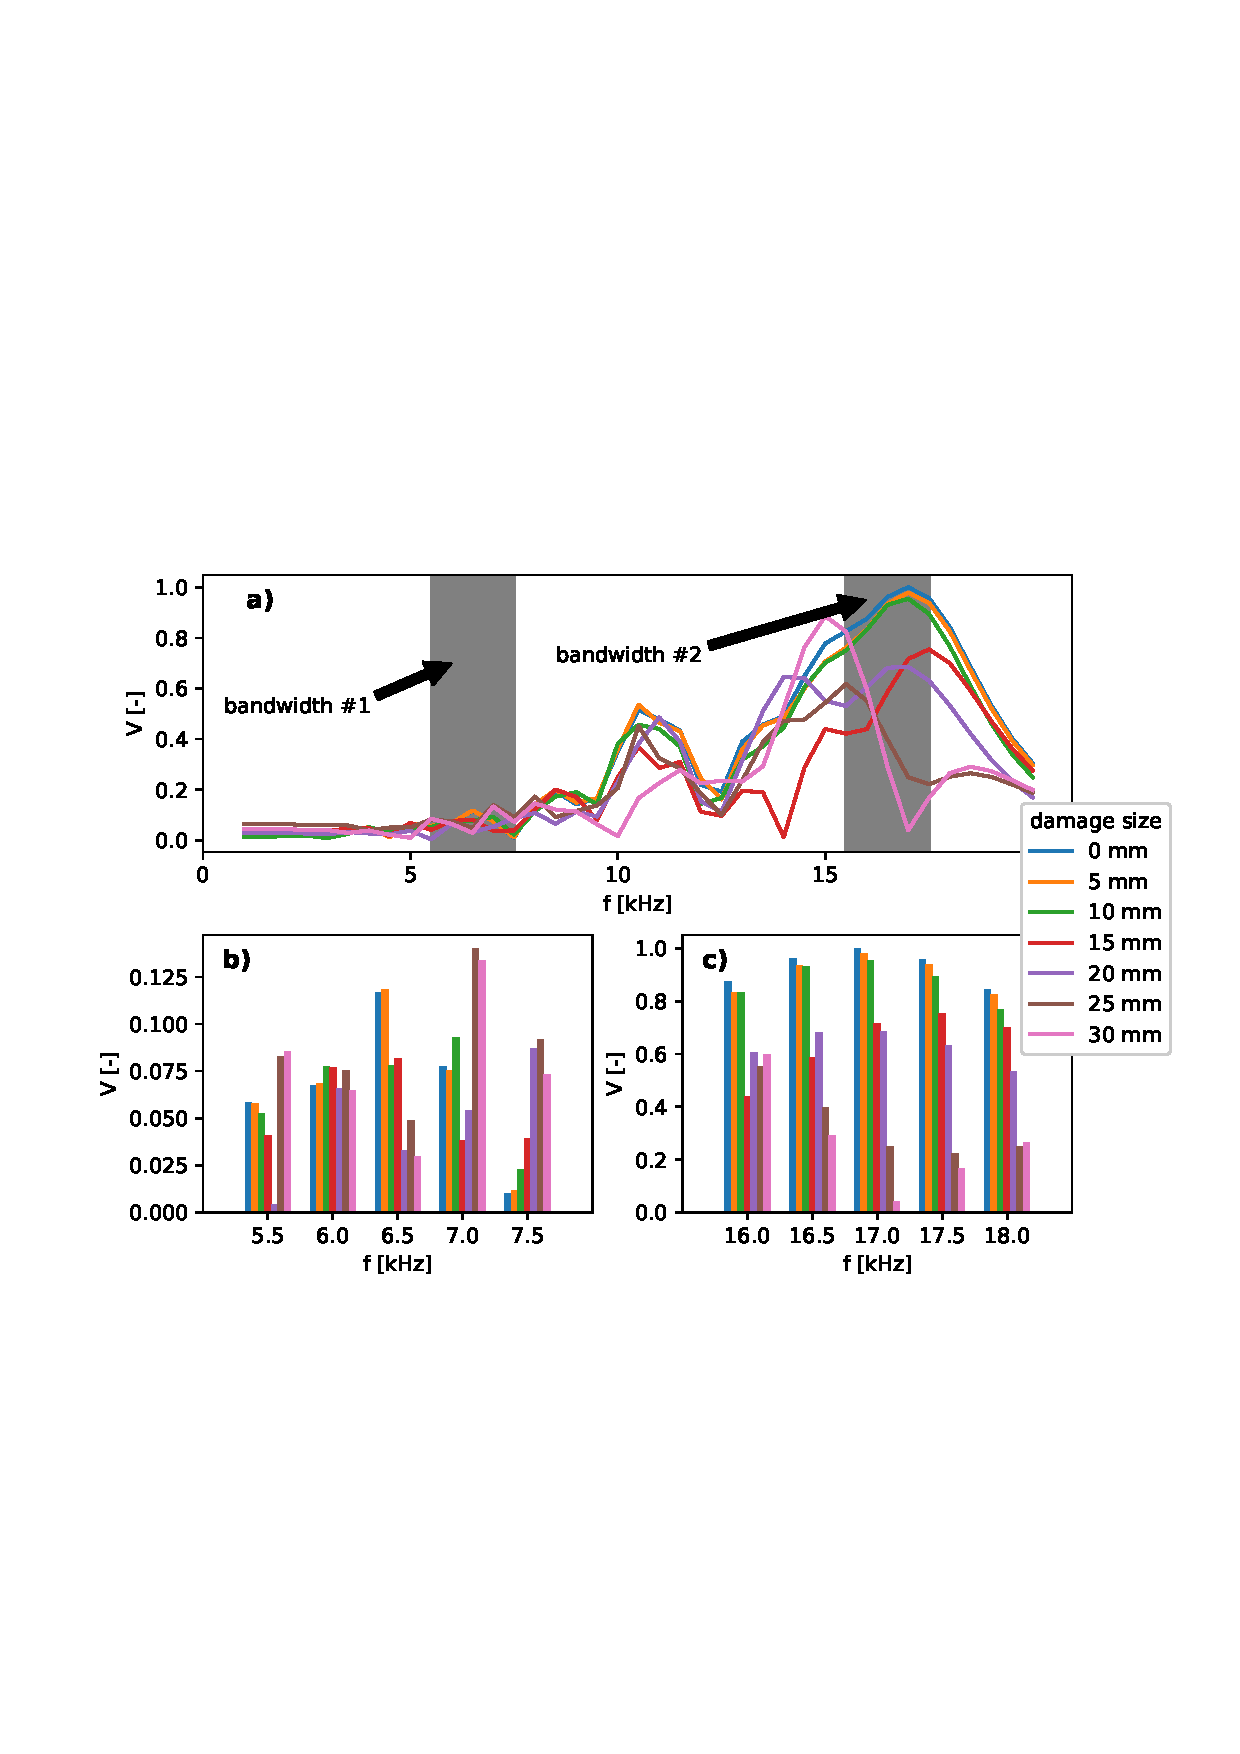
\includegraphics[width=1\linewidth]{../../../figures/pdf/time_fft.pdf}
	\end{center}
	\caption{The sensor signal in frequency domain a) full excitation bandwidth, b) bandwidth \#1, c) bandwidth \#2}
	\label{fig:signals}
\end{figure}
This assumption is fulfilled by the frequency 16.5 kHz (Fig. \ref{fig:signals}c)).
Moreover, normalized the MADIF values are within a wide range, i.e. 0.2--1.0 (Fig. \ref{fig:madif}).
\begin{figure}
	\begin{center}
		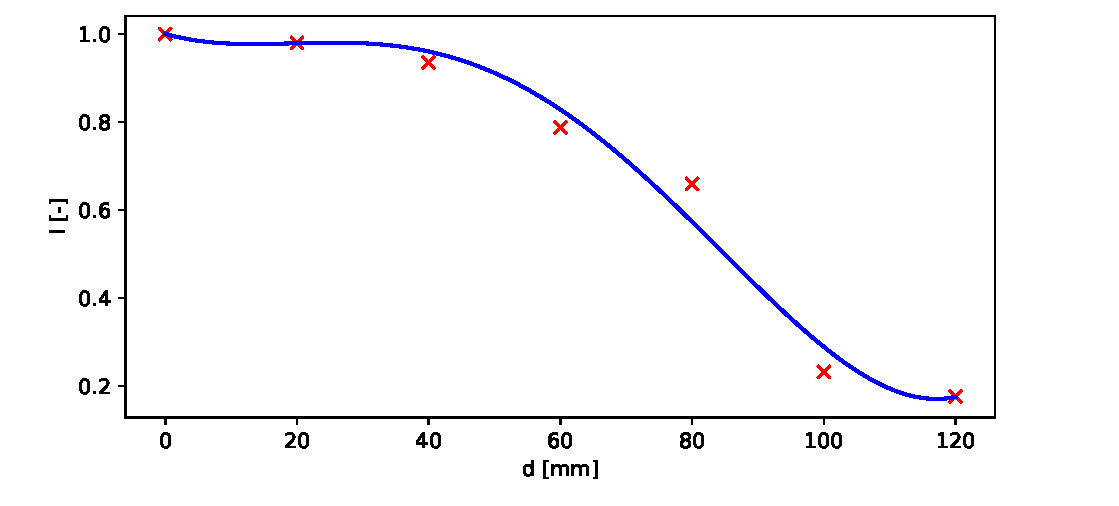
\includegraphics[width=1\linewidth]{../../../figures/eps/madif.eps}
	\end{center}
	\caption{madif}
	\label{fig:madif}
\end{figure}
This function can be used to identify damage to the physical sample associated with the model.
The severity of the failure shall be read from the determined characteristic for the value of the sensor voltage which has been measured according to the simulation scheme.

\section{Conclusions}
\label{sec:conc}
The paper presents the preliminary study on the possibility usage of model-assisted approach to identify a severity of damage in composite structures. 
numerical analysis of GW propagation in the sandwich composite panel.  
\appendix
\section{}
\label{app:matrices}
The formulae of matrices for 3D elements are:
\begin{eqnarray}
\textbf{M}_{dd}^e & = & \int_{V_e}\textbf{N}^T\rho \textbf{N}\rmd V_e\\
\textbf{K}_{dd}^e & = & \int_{V_e}{\textbf{B}_d^e}^T\textbf{c}\textbf{B}_d^e\rmd V_e
\end{eqnarray}
where \textbf{c} and \(\rho\) is the elasticity matrix and mass density, 
respectively and \(\int_{V_e}dV_e\) is a volume integral.

The formulae of matrices for 2D elements are:
\begin{eqnarray}
\textbf{M}_{dd}^e & = & 
\left [
\begin{array}{cc}
\textbf{M}_T^e & 0\\
0 & \textbf{M}_R^e
\end{array}
\right] =
\int_{\Omega_e}\textbf{N}^T\rho 
\left [
\begin{array}{cccccc}
h &  & &  &  &\\
0 & h & & & &\\
0 & 0 & h & & & \\
0 & 0 & 0 & \frac{h^3}{12} & &\\
0 & 0 & 0 & 0 & \frac{h^3}{12} &\\
0 & 0 & 0 & 0 & 0 & 0
\end{array} \right]
\textbf{N}\rmd \Omega_e\\
\textbf{K}_{dd}^e & = & \int_{\Omega_e}{\textbf{B}_b^e}^T
\left[
\begin{array}{cc}
\textbf{A} & \textbf{B}\\
\textbf{B} & \textbf{D}
\end{array} \right]
\textbf{B}_b^e\rmd \Omega_e+\int_{\Omega_e}{\textbf{B}_s^e}^T\textbf{A}^{\ast}\textbf{B}_s^e\rmd \Omega_e
\end{eqnarray}
where h is the element thickness and \(\int_{\Omega_e}d\Omega_e\) is a surface 
integral and:
\begin{eqnarray}
\textbf{A} & = & \textbf{c}_{ij}(h_t-h_b)\qquad i,j=1,2,6\nonumber\\
\textbf{B} & = & \frac{1}{2}\textbf{c}_{ij}(h_t^2-h_b^2)\qquad i,j=1,2,6\nonumber\\
\textbf{D} & = & \frac{1}{3}\textbf{c}_{ij}(h_t^3-h_b^3)\qquad i,j=1,2,6\nonumber\\
\textbf{A}^{\ast} & = & \kappa \, \textbf{c}_{ij}\left[h_a-4/3\left(h_t^3-h_b^3\right)/h_a^2\right]\qquad i,j=4,5\nonumber
\end{eqnarray}
where the \(h_t\) and \(h_b\) are the distance from mid-plane to the top and 
the bottom layer of the element, respectively and the \(\kappa=5/4\) is a shear 
correction factor.

The dielectric conductivity matrix \(\textbf{K}_{\phi \phi}^e\) and 
piezoelectric coupling matrix \(\textbf{K}_{u \phi}^e\) are defined:
\begin{eqnarray}
\textbf{K}_{d\phi}^e & = & \int_{V_e}{\textbf{B}_d^e}^T\textbf{e}^T \textbf{B}_{\phi}^e\rmd V_e\\
\textbf{K}_{\phi \phi}^e & = & -\int_{V_e}{\textbf{B}_{\phi}^e}^T 
{\textbf{\(\bepsilon\)}^S}^T \textbf{B}_{\phi}^e\rmd V_e
\end{eqnarray}

\section{}
\label{app:properties}
Mechanical properties of carbon fibres, epoxy resin and the adhesive layer are 
presented in a table~\ref{tab:properties} and evaluated effective elastic 
properties for a single layer in a table~\ref{tab:properties_layer}.
\begin{table}
\centering
\caption{\label{tab:properties}Material properties of carbon fibres, epoxy 
resin and the adhesive layer}
\begin{tabular}{ccccc}\hline
Material & \(E_{11}\) &  \(E_{33}\) & \(\nu_{12}\) & \(\rho\) \\
 & [GPa] &  [GPa] & [-] & [\(kg/m^3\)]\\
\hline
Carbon & 275.6 & 27.6 & 0.2 & 1900\\
Epoxy & 3.43 & 3.43 & 0.35 & 1250\\
Adhesive & 1.7 & 1.7 & 0.34 & 1200\\
\end{tabular}
\end{table}

\begin{table}
\centering
\caption{\label{tab:properties_layer}Effective material properties of a single 
layer}
\begin{tabular}{cccccccc}
\hline
 \(E_{11}\) & \(E_{22}\) & \(E_{33}\) & \(G_{12}\) & \(G_{23}\) & \(\nu_{12}\) 
 & \(\nu_{23}\) & \(\rho\) \\
\([\)GPa] & [GPa] & [GPa] & [GPa] & [GPa] & [-] & [-] & [\(kg/m^3\)]\\
\hline
137 & 8.7 & 8.7 & 3.61 & 3.19 & 0.28 & 0.37 & 1569\\
\hline
\end{tabular}
\end{table}


Material properties of the PZT transducer:
\begin{eqnarray}
\textbf{c}^E=\left [ 
\begin{array}{cccccc}
134 & 88.9 & 90.9 & 0 & 0 & 0 \\ 
88.9 & 134 & 90.9 & 0 & 0 & 0 \\
90.9 & 90.9 & 121 & 0 & 0 & 0 \\
0 & 0 & 0 & 20.5 & 0 & 0 \\
0 & 0 & 0 & 0 & 20.5 & 0 \\
0 & 0 & 0 & 0 & 0 & 22.4 \nonumber \\
\end{array}
\right ] \left [ GPa \right ] 
\end{eqnarray}
\begin{eqnarray}
\textbf{e}=\left[
\begin{array}{cccccc}
0 & 0 & 0 & 0 & 13.7 & 0\\
0 & 0 & 0 & 13.7 & 0 & 0\\
-6.06 & -6.06 & 17.2 & 0 & 0 & 0\nonumber \\
\end{array}
\right] \left[C\,m^{-2}\right]
\end{eqnarray}
\begin{eqnarray}
\bepsilon^S_r=\left[
\begin{array}{ccc}
906 & 0 & 0\\
0 & 906 & 0\\
0 & 0 & 823\nonumber \\
\end{array}
\right] \left[ - \right]
\end{eqnarray}
\begin{eqnarray}
\rho=7850\ [kg\,m^{-3}] \nonumber
\end{eqnarray}

\bibliography{../../../../../BibTex/Rozprawa}{}
\end{document}